\section{Handbuch}
  \label{sec:manual}

  \subsection{Systemvorraussetzungen \& Kompilation}

    Das Framework nutzt verschiedene Bibliotheken zum Testen, Generieren von
    Vektorbildern, Datenbankzugriff und zur Parsierung von
    Kommandozeilenparametern. Wir bedienen uns Maven2 als \emph{build tool}, um
    diese Abhängigkeiten automatisiert aufzulösen. Das Kompilieren wurde von
    uns ausschließlich unter GNU/Linux-Systemen getestet, jedoch sollte die
    Portierung nach Microsoft Windows leicht möglich sein. Vorraussetzungen
    für einen erfolgreichen Kompiliervorgang sind (in Klammern die Namen der Pakete
    bei Debian/Ubuntu-Systemen mit erfolgreich getesteten Versionsnummern):

    \begin{itemize}
      \item Java 1.6 Development Kit (\texttt{openjdk-6-jdk}, 
            Version \enquote{6b18-1.8.7-2~squeeze1})
      \item Maven 2 (\texttt{maven2}, Version 2.2.1-5)
    \end{itemize}

    Weiterführende Informationen zur Kompilierung des Projekts finden sich in
    der beiliegenden \texttt{README}-Datei.

  \subsection{Grafische Oberfläche}

    Die Oberfläche ermöglicht es Polygone zu generieren, Kürzeste Wege zwischen
    zwei Punkten zu berechnen und diese darzustellen.\\

    \begin{center}
      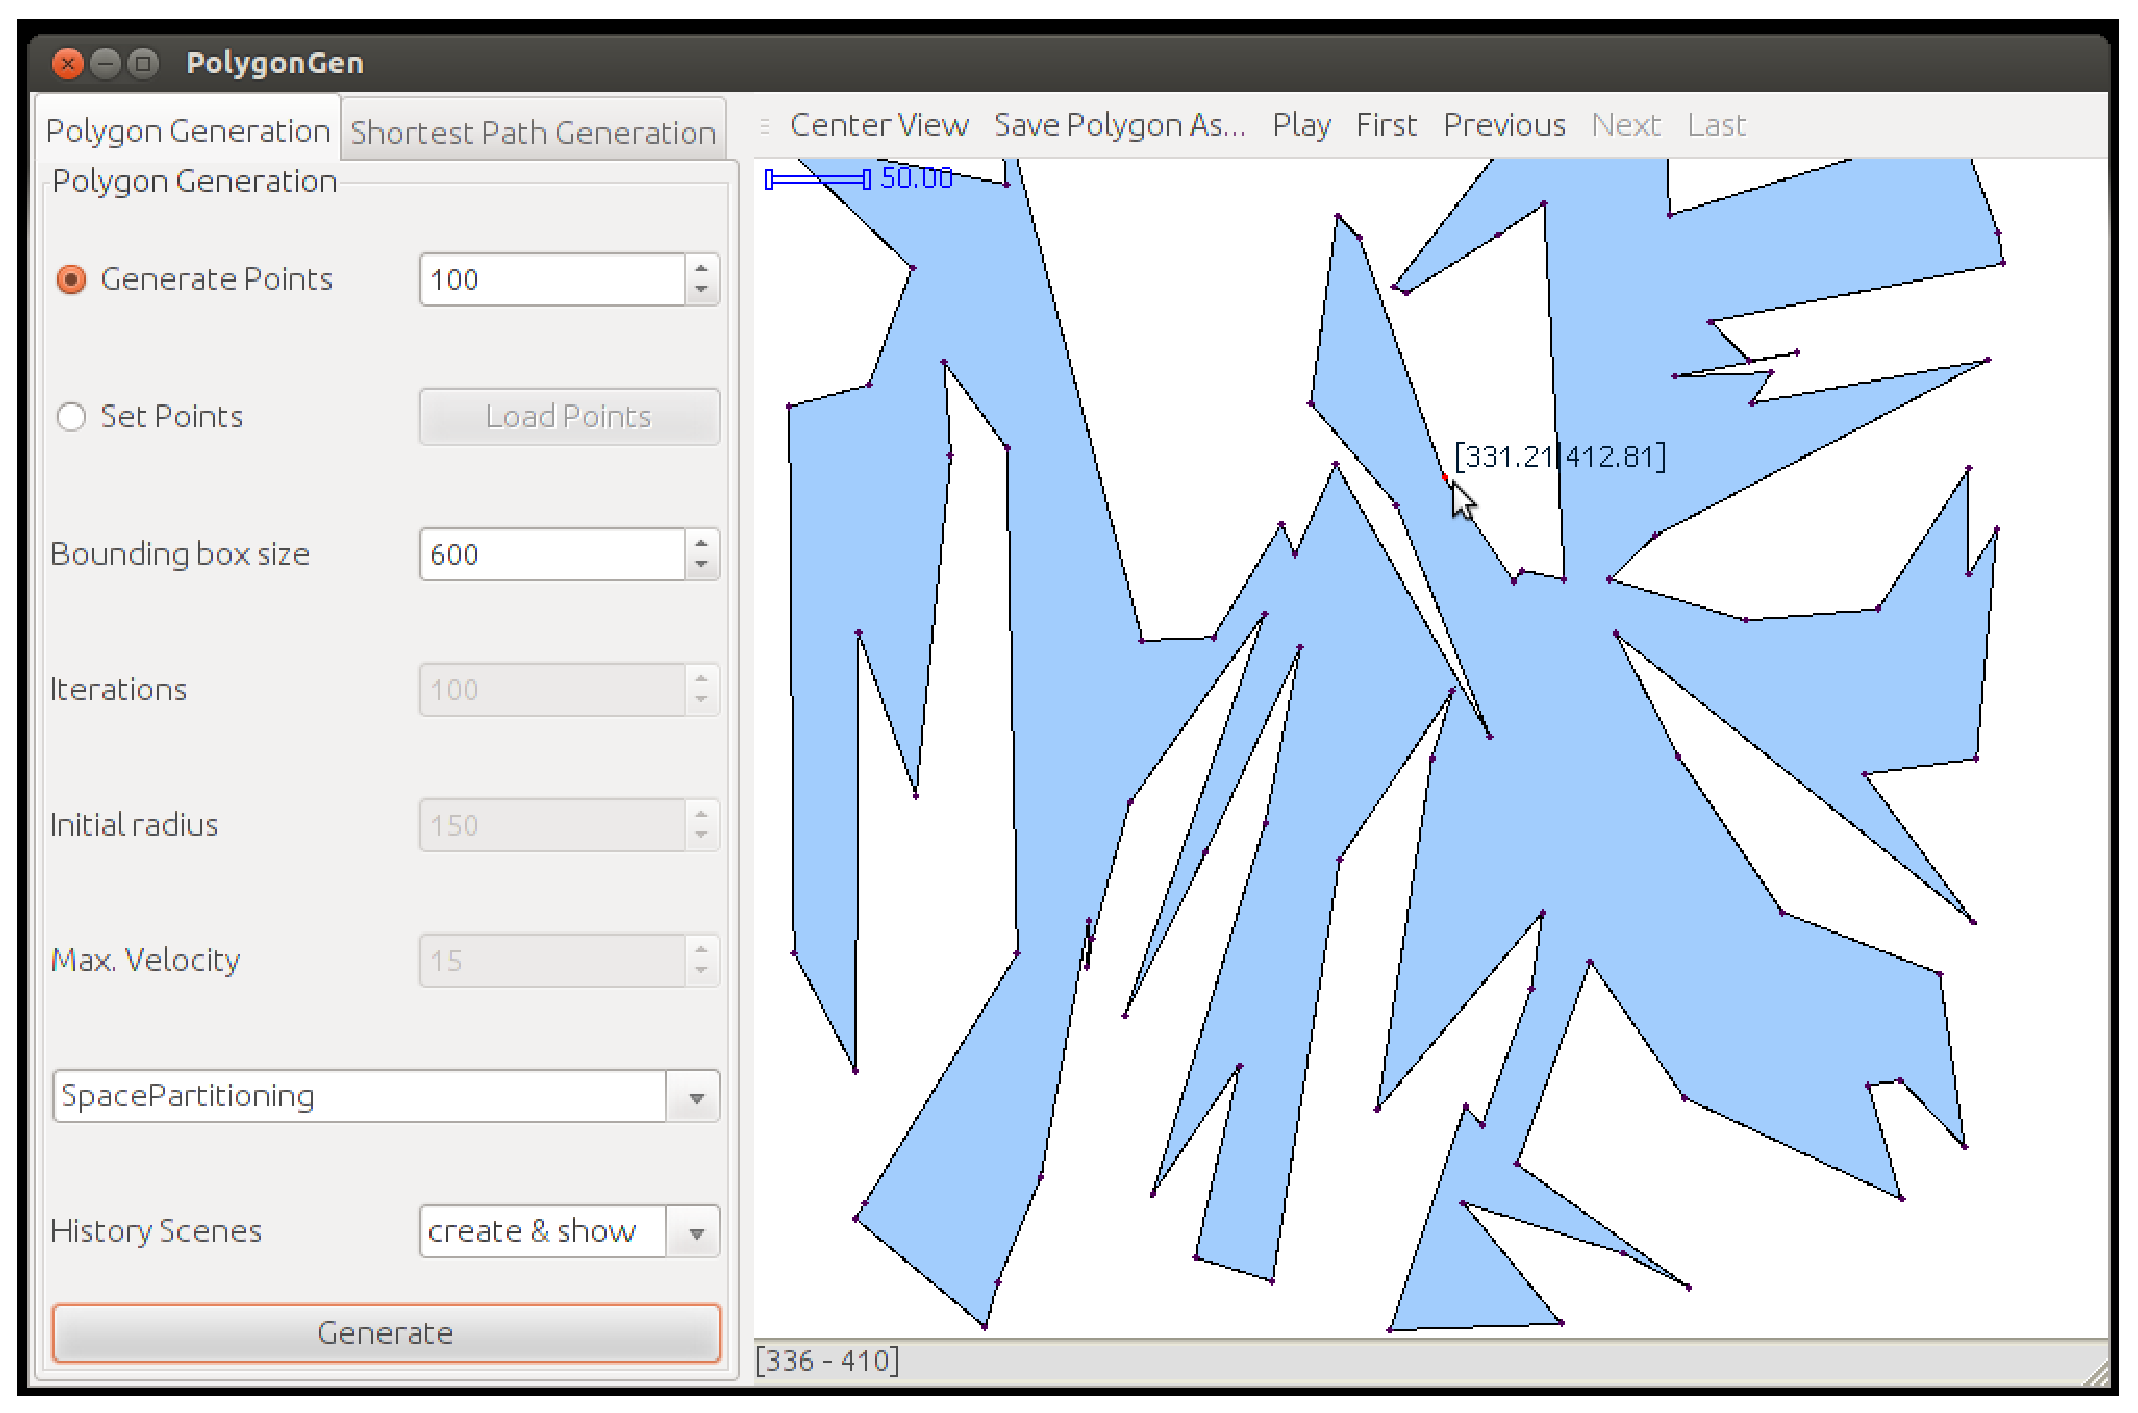
\includegraphics[width=0.7\textwidth]{img/GUI.eps}
    \end{center}

    \subsubsection{Funktionen}

      \begin{itemize}
        \item Generierung von Polygonen
        \item Visualisierung der Polygon-Algorithmen
        \item Manuelle Auswahl der Punktmenge eines Polygons
        \item Zoomen und Bewegen
        \item Anzeigen der Koordinaten einzelner Punkte
        \item Berechnung des Shortest-Path
        \item Speichern eines Polygons im CSV- oder SVG-Format
      \end{itemize}

  \subsection{Kommandozeile}

    Mit der Kommandozeile ist es möglich mehrere Polygone und deren Statistiken
    gleichzeitig zu erzeugen und diese auf der Kommandozeile auszugeben oder in
    eine CSV-Datei bzw. Sqlite Datenbank zu schreiben.
    Zusätzlich ist es möglich die Anzahl der Threads zu bestimmen für optimales
    paralleles Berechnen. Damit ist es möglich viele verschiedene Polygone mit
    den gleichen Parametern zu erzeugen. Die Parameter werden im \enquote{GNU-
    Stil} angegeben.\\ Um die Usage-Hilfe anzuzeigen, ruft man das Programm mit
    dem Parameter --help oder --usage auf. Listing~\ref{listing_usage} zeigt
    einen gekürzten Ausschnitt aus der Usage. Alle weiteren Parameter sind in
    der Usage näher erläutert.

\begin{code}[caption={Usage der Kommandozeile},label=listing_usage]
usage: run.sh [--algorithm <Algorithm>] [--boundingbox <boundingbox>]
       [--database <Database path>] [--help] [--no-header]
       [--no-statistics] [--number <Number of polygons>] [--output <Output
       path>] [--points <Number of points>] [--radius <circle radius>]
       [--runs <number of runs>] [--threads <Number of threads>] [--usage]
       [--velocity <velocity>]
-
Use with no arguments to show GUI.
--database will override --output, if neither is given, csv output will be
directed to console.-
    --algorithm <Algorithm>         The algorithm to execute, specified by
                                    ID (Default: 0). Available algorithms:
                                    [0] SpacePartitioning
                                    [1] Permute & Reject
                                    [2] 2-Opt moves
                                    [3] RandomPolygonAlgorithm
                                    [4] Incremental Construction &
                                    Backtracking
                                    [5] ConvexHull
                                    [6] Velocity Virmani
                                    [7] SteadyGrowth
                                    [8] TwoPeasants
                                    [9] Enumerating Permute & Reject

[...]
\end{code}

\begin{code}[caption={Beispiel-Ausführung},label=listing_usage_example]
\$ run.sh --algorithm 0 --number 10 --points 25 --output out
\end{code}

    Das Beispiel-Kommando in Listing~\ref{listing_usage_example} führt zur
    Generierung von 10 Polygonen mit je 25 Punkten mit Hilfe des \emph{Space
    Partitioning}-Algorithmus. Die erzeugten Polygone werden mitsamt der
    generierten Meta-Daten in die Datei out geschrieben.

  \subsection{Ausgabe}
    Ohne angabe weiterer Optionen werden generierte Polygone samt ihrer
    Meta-Daten auf Kommandozeile im CSV-Format ausgegeben. In der ersten Zeile
    sthet hierbei der Header für die entsprechenden Spalten der Ausgabe.

    \begin{itemize}
      \item \emph{polygon}\\
        Die Punkte des erzeugten Polygons als gegen den Uhrzeigersinn geordnete 
        Liste.
      \item \emph{used\_algorithm}\\
        Der zur Erzeugung des Polygons verwendete Algorithmus.
      \item \emph{number\_of\_points}\\
        Die Anzahl der Punkte im Polygon.
      \item \emph{surface\_area}\\
        Der Flächeninhalt des Polygons.
      \item \emph{circumference}\\
        Der Umfang des Polygons.
      \item \emph{timestamp}\\
        Unix-timestamp zur Erzeugungszeit des Polygons.
      \item \emph{time\_for\_creating\_polygon}\\
        Zur Generierung benötigte Zeit.
      \item \emph{iterations}\\
        Permute \& Reject: Die Anzahl der zu Erzeugung des Polygons benötigten 
        Durchläufe, d.h. es wurden iterations-1 Polygone als nicht einfache 
        Polygone zurückgewiesen.\\
        Velocity: Gleicht dem gleichnamigen Parameter.
      \item \emph{rejections}\\
        %TODO: kadir
        Velocity:
      \item \emph{count\_of\_backtracks}\\
        Incremental Construction and Backtracking: Die Anzahl der 
        durchgeführten Backtracks.
      \item \emph{radius}\\
        Velocity: Gleicht dem gleichnamigen Parameter.
      \item \emph{avg\_velocity\_without\_collisions}\\
        %TODO: kadir
        Velocity:
      \item \emph{initializeRejections}\\
        %TODO: kadir
        Velocity:
      \item \emph{maximumRejections}\\
        %TODO: kadir
        Velocity:
    \end{itemize}

    Die meisten Algorthmen generieren nur einen Teil der möglichen Meta-Daten.
    In diesem Fall wird \enquote{null} in die entsprechende Spalte eingetragen.
    Unter Angabe von \emph{--no-header} entfällt der Header als erste Zeile,
    durch \emph{--no-statistics} werden ausschliesslich die erzeugten Polygone
    ausgegeben, die Meta-Daten entfallen.

    Die Option \emph{--database <Database path>} bewirkt, dass die Ausgabe in
    eine Sqlite-Datenbank ensprechend des angegebenen Pfads geschrieben wird.
    Hierbei werden ausschliesslich die Meta-Daten gespeichert, um eine
    statistische Auswertung zu ermöglichen. Die erzeugte Tabelle entspricht der
    üblichen ausgabe, die Option \emph{--no-header} wird nicht beachtet.
